\documentclass{assignment}

\usepackage{float}
\usepackage{tikz}
\usepackage{adjustbox}
\usepackage{titlesec}
\usepackage{soul}
\usepackage{csvsimple}

\usepackage{graphicx}
\usepackage{subcaption}
\usetikzlibrary{shapes, arrows}

\usetikzlibrary{calc,patterns,angles,quotes}
\setlength{\parindent}{0pt}

\hypersetup{
pdftitle={ME663 - Computational Fluid Dynamics},
pdfsubject={Personal project report},
pdfauthor={Tommaso Bocchietti}
}

\title{Post Flight Drag Coefficient Analysis of a Model Rocket Using Ansys Fluent}
\author{Tommaso Bocchietti}
\date{A.Y. 2023/24 - W24}


\begin{document}

\maketitle

\begin{figure}[H]
	\centering
	
\includegraphics[width=.9\textwidth]{./pdf/UniversityOfWaterloo_logo_vert_pms}
	\label{fig:University_Of_Waterloo_logo}
\end{figure}

\vspace*{\fill}

Personal project report. \\

Instructor: Prof. Fue-Sang Lien \\
Course: ME663 - Computational Fluid Dynamics \\
Term: Winter 2024 \\

\clearpage
\tableofcontents

\clearpage
\listoffigures
\listoftables
\lstlistoflistings
% \printglossary[type=\acronymtype]

\clearpage
\section{Introduction}

Every electronic device requires the use of a timing system (usually referred as clock) that sets the reference for the operation of the device.
This timing system is implemented through the use of various electronic components such as clock source, phase comparator, frequency dividers, \dots.

The aim of this project is to investigate the state of the art of clock sources technologies, with a focus on the most recent advancements in the field and their potential applications.
In particular, the project will focus on the following topics:

\begin{itemize}
    \item \semph{Crystal oscillators}: electric oscillator type circuit that uses a piezoelectric resonator, a crystal, as its frequency-determining element (\href{https://en.wikipedia.org/wiki/Crystal_oscillator#Terminology}{Wikipedia definition}).
    \item \semph{\acrshort{mems} resonators}: small electromechanical structures that vibrate at high frequencies (\href{https://en.wikipedia.org/wiki/Microelectromechanical_system_oscillator#Resonators}{Wikipedia definition}).
    \item \semph{\acrshort{mems} Atomic Clocks} (time permitting): the combination of a \acrshort{mems} system fabrication with atomic clocks for small, cheap, low-power devices \cite{KNAPPE2008571}.
\end{itemize}



\section{Methodology}
\label{sec:methodology}

We will start by writing the analytical expression of the \textbf{shape functions} for the 4-node element with total length $h_e$ and $\alpha = \beta = \frac{1}{3}$ in terms of the parent coordinate system, $-1 \leq \xi \leq 1$.
To do so, we will make use of \texttt{Mathematica} to perform the symbolic computation and obtain the exact expression of the shape functions.

We will proceed by writing the elemental matrices ($B_0^e$, $f_{int}^e$, $f_{ext}^e$, $f_{kin}^e$) still in terms of the parent coordinate system.

We will then write the \textbf{MATLAB} code to solve the problem implementing the explicit integration scheme with Total Lagrangian finite element formulation and finally plot the deformation of the right end of the bar vs time, namely $u_{end}(t)$.
\section{CAD modeling}
\label{sec:cad_modeling}

The first step in the analysis is to create the CAD of the model rocket.

Any CAD software can be used to create the model but for this project we used \texttt{CATIA V5}.

To simplify the analysis, some details of the rocket were omitted from the CAD model, such as the launch lug or the nozzle of the engine.
We believe that these simplifications do not affect the accuracy of the study, as the focus is on the nose cone, body, and fins of the rocket.

In Figure \ref{fig:CAD_model_drawing}, the technical drawing of the model is shown, along with the main dimensions.

\begin{figure}[H]
    \centering
    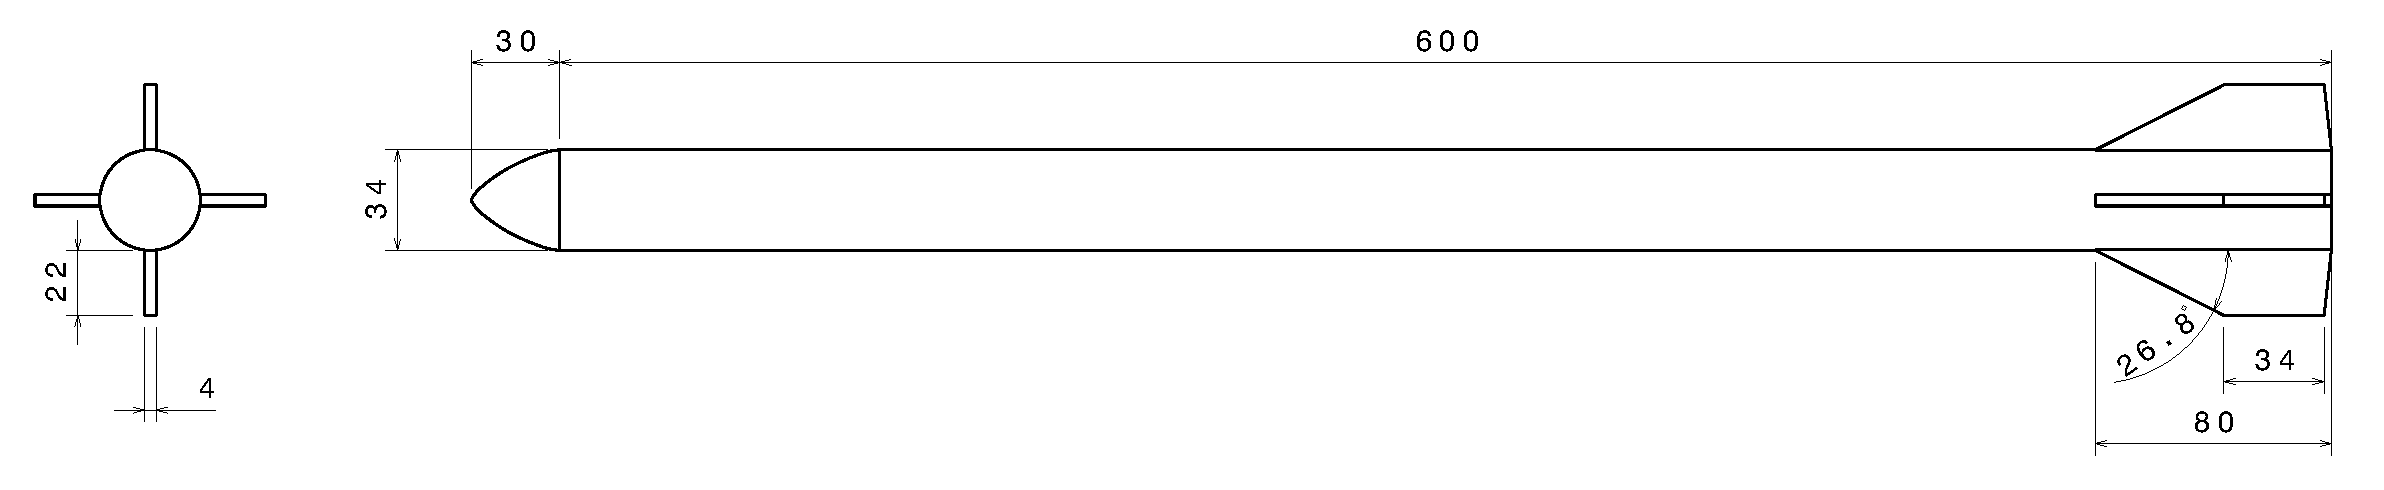
\includegraphics[width=\textwidth]{pdf/CAD_drawing.pdf}
    \caption{CAD model of the model rocket analyzed in this project. Measurements are in millimeters.}
    \label{fig:CAD_model_drawing}
\end{figure}

Probably the most important part of the CAD model is the choice of the nose cone shape.
For this project, we decided to adopt the \textbf{Haack series} nose cone, which is a common choice for model rockets.
In particular, instead of being geometrically defined, the Haack series nose cones are mathematically derived to minimize drag.
The shape is controlled by a parameter $C$, which can be set to different values to obtain different nose cone shapes.
The equations that defines the Haack series nose cone are:

\begin{align}
    \theta(x)    & = \arccos\left(1 - \frac{2x}{L}\right)                                            \\
    y(\theta, C) & = \frac{R}{\sqrt{\pi}} \sqrt{\theta - \frac{\sin{2\theta}}{2} + C \sin^3{\theta}} \\
\end{align}

Where $L$ is the length of the nose cone, $R$ is the radius of the base, and $C$ is the parameter that controls its shape.

In our case, we opted for a Haack series nose cone with $C = 0$, which is known to minimize the drag for a given length and diameter.
This choice is common in model rocketry, and can also be found under the name of \textbf{LD-Haack (Von Kármán)} nose cone.

\begin{figure}[H]
    \centering
    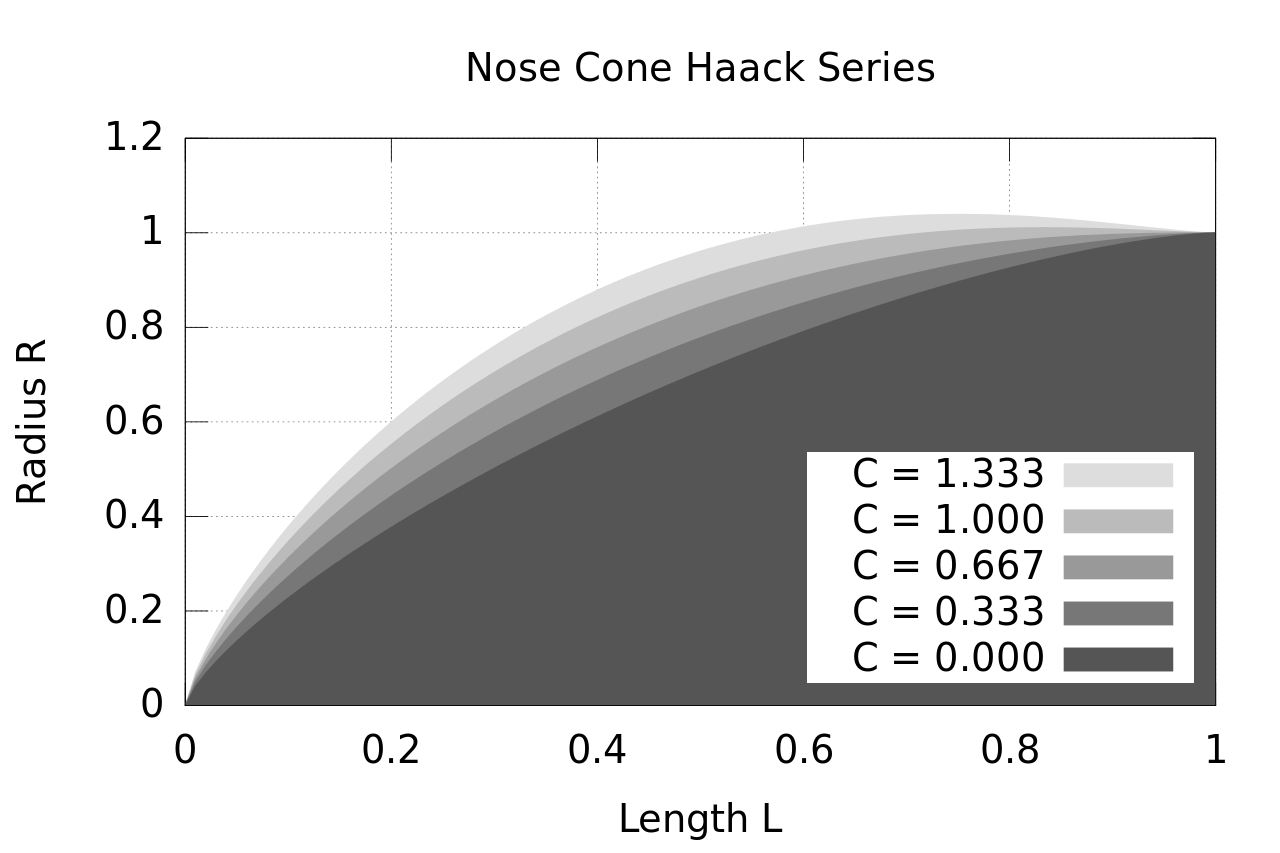
\includegraphics[width=.6\textwidth]{img/Nose_Cone_Haack_Series.png}
    \caption{Haack series nose cone with $L = 1$, $R = 1$, and different values of $C$.}
    \label{fig:LD_Haack_nose_cone}
\end{figure}
\section{CFD simulation}
\label{sec:cfd_simulation}

The second step in the analysis is to perform the CFD simulations of the model rocket.

Before running the actual simulations however, we need to perform a series of preliminary steps to prepare the model.

\subsection{Geometry preparation}
\label{subsec:geometry_preparation}

The first step in the CFD simulation is to prepare the geometry of the model rocket and import it into \texttt{DesignModeler} of \texttt{Ansys Fluent}.

Once the main geometry is imported, we need to create the computational domain around the rocket.
For this study, we opted for a simple rectangular domain, with a length of $1.5m$ ($0.5m$ in front of the rocket and $1m$ behind it) and a height and width of $0.7m$ (see Figure \ref{fig:rocket_geometry}).

\begin{figure}[H]
    \centering
    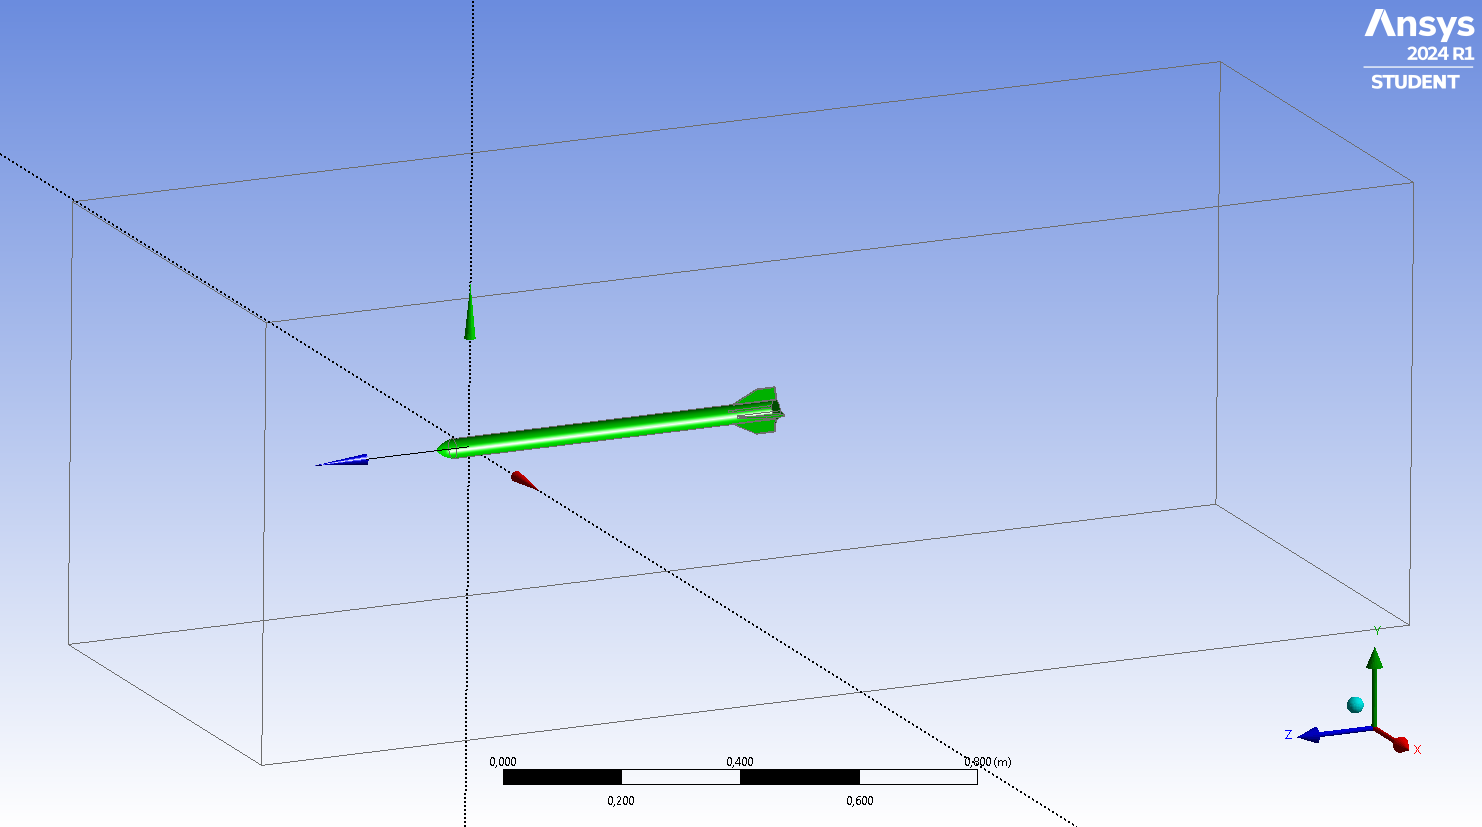
\includegraphics[width=.7\textwidth]{img/DesignModeler.png}
    \caption{Geometry of the model rocket and the surrounding domain in \texttt{DesignModeler}.}
    \label{fig:rocket_geometry}
\end{figure}

The choice in the size of the domain was driven by the idea of having enough space around the rocket to allow the flow to develop and avoid any boundary effects that could affect the results.
In fact, the domain distance in the radial direction from the rocket is about 10 times ($0.7/2 = 0.35 \approx 0.34 = 10 * 0.034$) the diameter of the rocket, which is a common rule of thumb for the size of the domain in CFD simulations.

\subsection{Mesh generation}
\label{subsec:mesh_generation}

The next step in the CFD simulation is to generate the mesh for the computational domain.

Given that our focus is strictly related to the rocket itself and not the flow field around it, we opted for a relatively coarse mesh at the boundary of the domain, and a progressively finer mesh around the rocket.
Having the possibility to do so, we also opted for an unstructured mesh, which allows for a more accurate representation of the geometry at the cost of a higher computational time (manageable in our case given the relatively small size of the domain).

The mesh was generated using \texttt{Mechanical} module.
Default parameters were used for the mesh generation, except of the \textit{Inflaction Layer Mesh} around the rocket.

In Table \ref{tab:mesh_inflaction} we report the parameters that were changed from the default values for the mesh generation around the rocket.

\begin{table}[H]
    \centering
    \begin{tabular}{|r|c|}
        \hline
        \textbf{Parameter}      & \textbf{Value}        \\
        \hline
        Use Automatic Inflation & Program Controlled    \\
        Inflation Option        & First Layer Thickness \\
        First Layer Height      & $1.5^{-3}m$           \\
        Maximum Layers          & $20$                  \\
        Growth Rate             & $1.2$                 \\
        Inflation Algorithm     & Pre                   \\
        View Advanced Options   & No                    \\
        \hline
    \end{tabular}
    \caption{Mesh \textit{Inflation} parameters used.}
    \label{tab:mesh_inflaction}
\end{table}

In Table \ref{tab:mesh_statistics} we report the statistics of the generated mesh.

\begin{table}[H]
    \centering
    \begin{tabular}{|c|c|}
        \hline
        \textbf{Parameter} & \textbf{Value} \\
        \hline
        Number of Nodes    & $73473$        \\
        Number of Elements & $177218$       \\
        \hline
    \end{tabular}
    \caption{Mesh statistics.}
    \label{tab:mesh_statistics}
\end{table}

\begin{figure}[H]
    \centering
    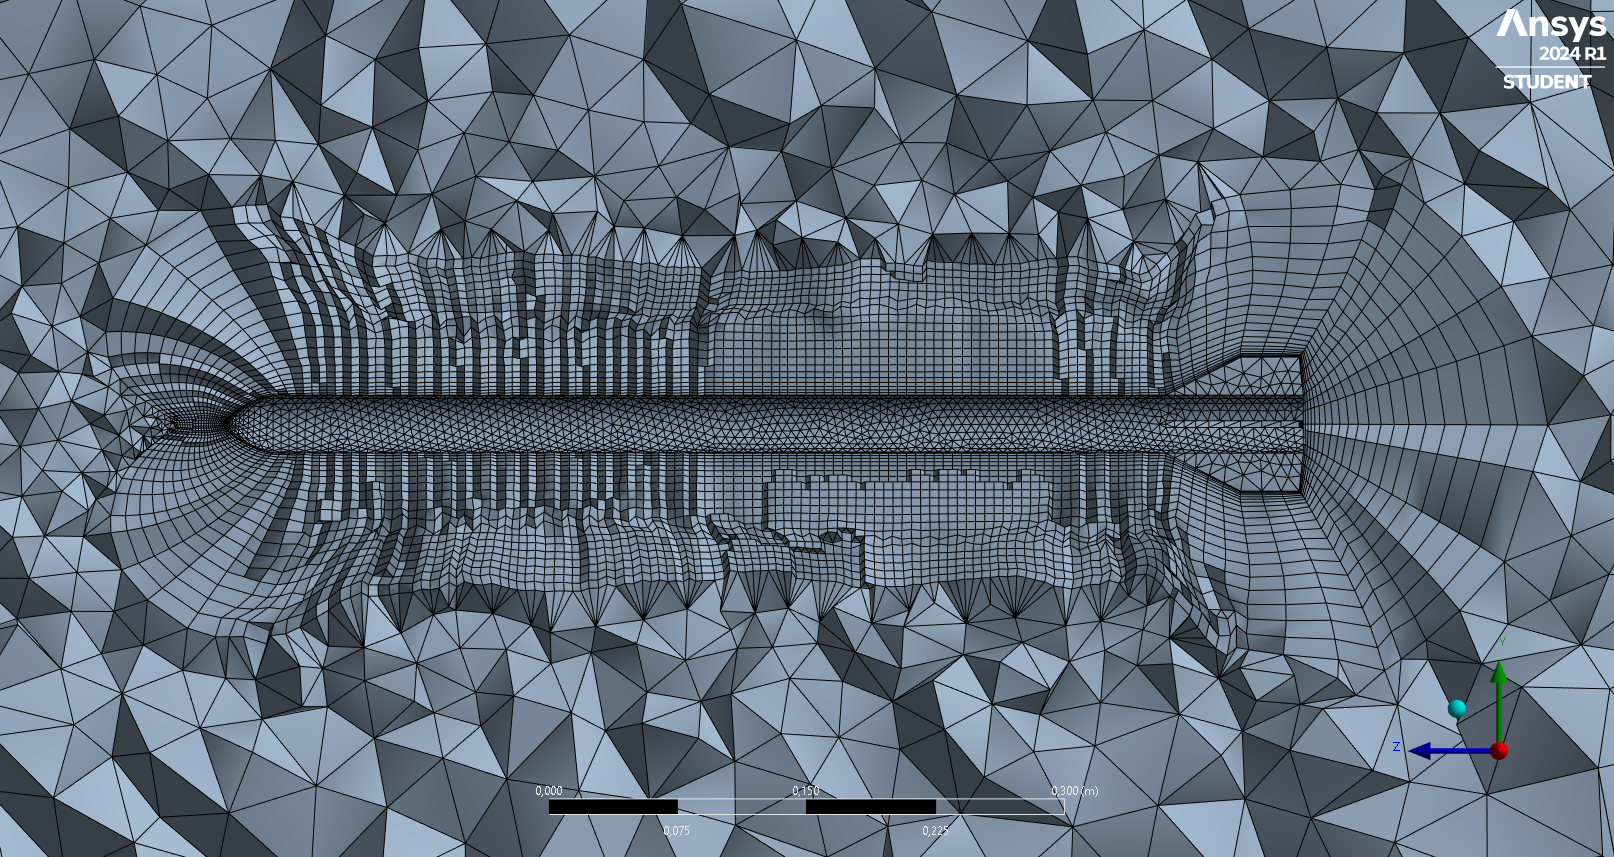
\includegraphics[width=.7\textwidth]{img/PreRunning/Mesh_sectioned.png}
    \caption{The inflation layer mesh around the rocket body is clearly visible.}
    \label{fig:mesh_sectioned}
\end{figure}

\begin{figure}[H]
    \centering
    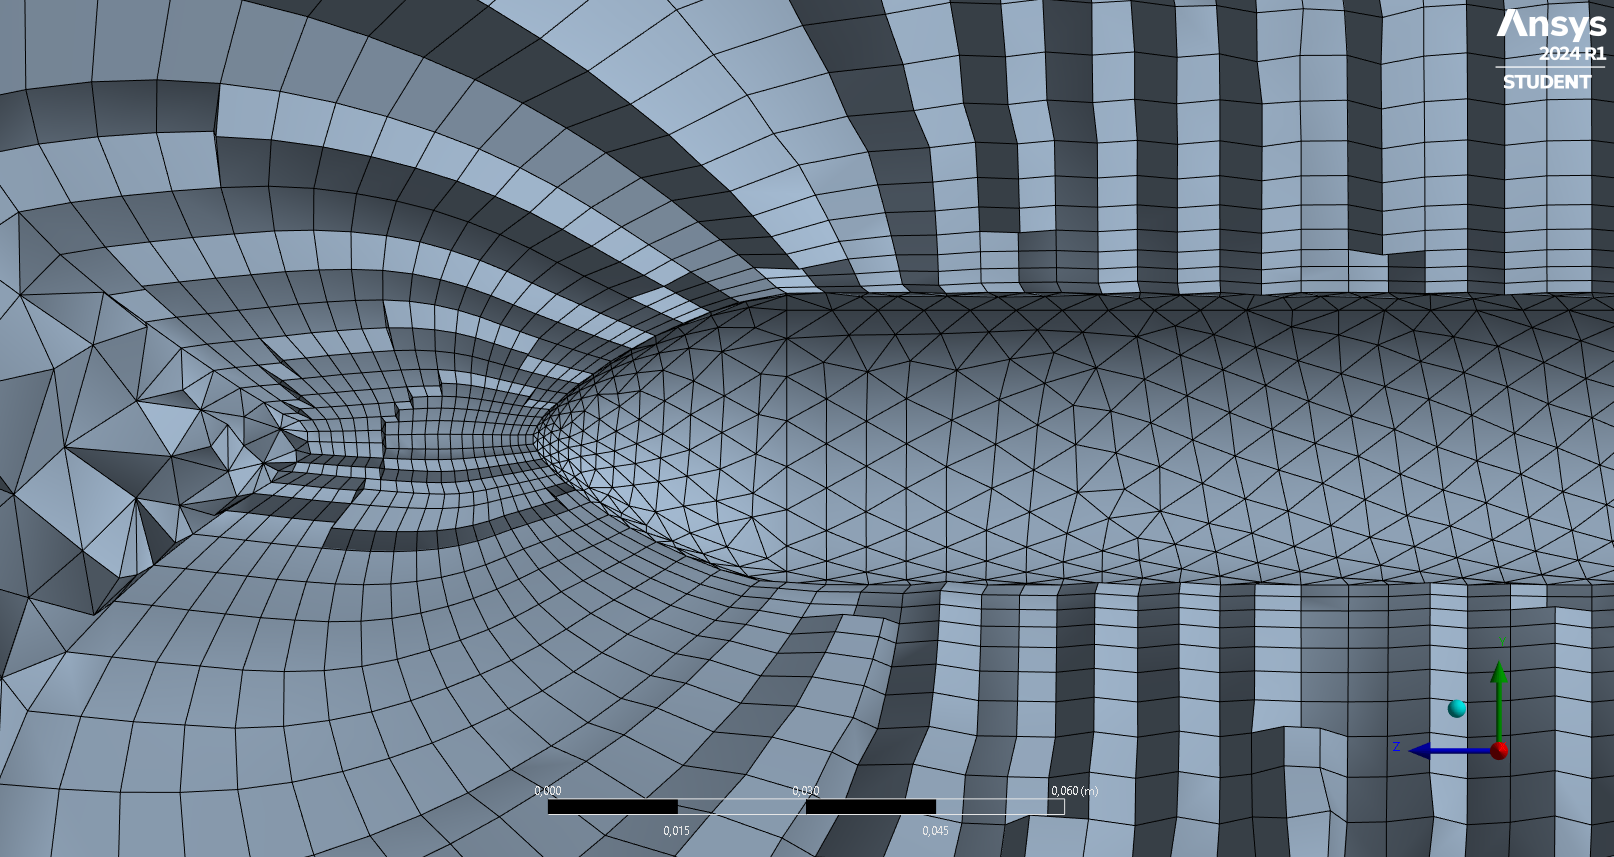
\includegraphics[width=.7\textwidth]{img/PreRunning/Mesh_sectioned_nose.png}
    \caption{Mesh details around the rocket nose cone. Due to the relatively high curvature of the nose cone, the generated mesh is finer with respect to the linear element of the rocket body.}
    \label{fig:mesh_sectioned_nose}
\end{figure}
\subsection{Fluent setup}
\label{subsec:fluent_setup}

The next step in the CFD simulation is to set up \texttt{Fluent} solver.

Here, many configurations could be set, such as the turbulence model, the solver type, the discretization scheme, etc.
Given our inexperience with CFD simulations, we opted for the default settings for most of the parameters with some exception that are reported in the following subsections.


\subsubsection{Turbulence model}
\label{subsubsec:turbulence_model}

One of the most important parameters to set in the CFD simulations is the turbulence model.

The turbulence model is a mathematical model used to predict the effects of turbulence on the flow field.
In our case, we opted for the \textit{k-$\omega$ SST} model, which is a widely used model for external aerodynamics simulations.

The SST \textit{k-$\omega$} model is a two-equation eddy-viscosity model that basically combines both the \textit{k-$\omega$} and \textit{k-$\epsilon$} models.
The use of this model allows for a good prediction of the flow field around the rocket, especially in the near-wall regions and transitional flows.

To do so, we use a \textit{k-$\omega$} model in the inner parts of the boundary layer, making the model directly usable all the way down to the wall through the viscous sub-layer, hence the SST \textit{k-$\omega$} model can be used as a Low-Re turbulence model without any extra damping functions.
The SST formulation also switches to a \textit{k-$\epsilon$} behaviour in the free-stream, avoiding the common \textit{k-$\omega$} problem that the model is too sensitive to the inlet free-stream turbulence properties.

Refer to Menter \cite{Menter1994TwoequationET} for more details on the SST \textit{k-$\omega$} model.


\subsubsection{Report definition}
\label{subsubsec:report_definition}

In the \texttt{Fluent} solver, it is possible to define the reports that will be generated during the simulation.

In our case, we have defined a custom report for the computation of the drag coefficient.
The only parameter that we had to modify to enhance the accuracy, was the reference area.

For a simple model rocket, the reference area can be considered as the largest cross-sectional area of the body tube.
In our case:

\begin{equation}
    A_{\text{ref}} = \pi \cdot \left( \frac{D}{2} \right)^2 = 0.0009079203 \quad [m^2]
\end{equation}



\subsection{Compressibility effects}
\label{subsec:compressibility_effects}

Before moving on, we need to decide whether to take into account the compressibility effects in the simulations or not.

It's well known from literature and experimental data that compressibility effects start to become important when the flow speed reaches a significant fraction of the speed of sound.
In particular, the Mach number of the flow is a good indicator of the importance of the compressibility effects.
The condition that distinguishes between incompressible and compressible flows is given by:

\begin{equation}
    Ma = \frac{v}{c} = \begin{cases}
        < 0.3 & \text{Incompressible flow} \\
        > 0.3 & \text{Compressible flow}
    \end{cases}
    \label{eq:mach_number}
\end{equation}

Where $Ma$ is the Mach number, $v$ is the flow speed and $c$ is the speed of sound in the fluid.

To determine whether to take into account the compressibility effects or not, we need to make some hand calculations based on the whether condition present when the rocket was flying.
In Table \ref{tab:conditions} we report the relevant parameters.

\begin{table}[H]
    \centering
    \begin{tabular}{|c|c|}
        \hline
        \textbf{Parameter} & \textbf{Value} \\
        \hline
        Altitude           & $1444m$        \\
        Temperature        & $15^{\circ}C$  \\
        \hline
    \end{tabular}
    \caption{Conditions present during the rocket flight.}
    \label{tab:conditions}
\end{table}

Considering air as an ideal gas, the definition of the speed of sound is given by the following equation:

\begin{equation}
    c = \sqrt{\gamma \frac{p}{\rho}} = \sqrt{\gamma \bar{R} T}
    \label{eq:speed_of_sound}
\end{equation}

Where $\gamma$ is the specific heat ratio, $\bar{R}$ is the specific gas constant and $T$ is the temperature of the fluid.

The specific heat ratio for air is $\gamma = 1.4$ and the specific gas constant considering dry air can be computed as:

\begin{equation}
    \bar{R} = \frac{R}{M_{mol}} = \frac{8.314}{\frac{28.96}{1000}} = 287.05 \frac{J}{kg \cdot K}
\end{equation}

Where $R$ is the universal gas constant and $M_{mol}$ is the molar mass of dry air.

Plugging the values into Equation \ref{eq:speed_of_sound}, we get:

\begin{equation}
    c = \sqrt{1.4 \cdot 287.05 \cdot (273.15 + 15)} = 340.3 \frac{m}{s}
\end{equation}

From the rocket flight data, we know that the rocket reached a maximum speed of around $130m/s$.

Plugging the values into Equation \ref{eq:mach_number}, we get:

\begin{equation}
    Ma = \frac{130}{340.3} = 0.382
\end{equation}

The maximum Mach number is $0.382$, which is above the threshold of $0.3$.
For this reason, we decided to take into account the compressibility effects in the simulations.
To do so, we modified the \textit{Material} properties in \texttt{Fluent}, setting the model of the air to \textit{Ideal Gas} instead of \textit{Incompressible}.

However, we believe that this choice is not critical for the results of the simulations, given that the maximum Mach number was reached only for a short period of time during the flight, while for the rest of it $Ma$ was below the threshold.

\subsection{Boundary conditions}
\label{subsubsec:boundary_conditions}

We now need to set the boundary conditions for the simulations.

The boundary conditions types used for the simulations are reported in Table \ref{tab:boundary_conditions}.

\begin{table}[H]
    \centering
    \begin{tabular}{|c|c|}
        \hline
        \textbf{Boundary} & \textbf{Condition type} \\
        \hline
        Inlet             & Velocity Inlet          \\
        Outlet            & Pressure Outlet         \\
        Rocket Surface    & Wall                    \\
        Domain Surface    & Wall                    \\
        \hline
    \end{tabular}
    \caption{Boundary conditions type used for the CFD simulations.}
    \label{tab:boundary_conditions}
\end{table}


\paragraph{Velocity inlet}

Since our target here is to obtain a drag coefficient that is representative of the average flight conditions, we decided to reduce the speed to $85\%$ of the maximum one.
Based on the data collected from the performed flight, we know that the rocket reached a maximum speed of $\approx 127m/s$.
By computing $85\%$ of this value, we get a speed of $\approx 110m/s$.

This is a strong approximation, given that the drag coefficient $C_d$ is also function of the speed of the flow (see Figure \ref{fig:velocity_inlet}).

\begin{figure}[H]
    \centering
    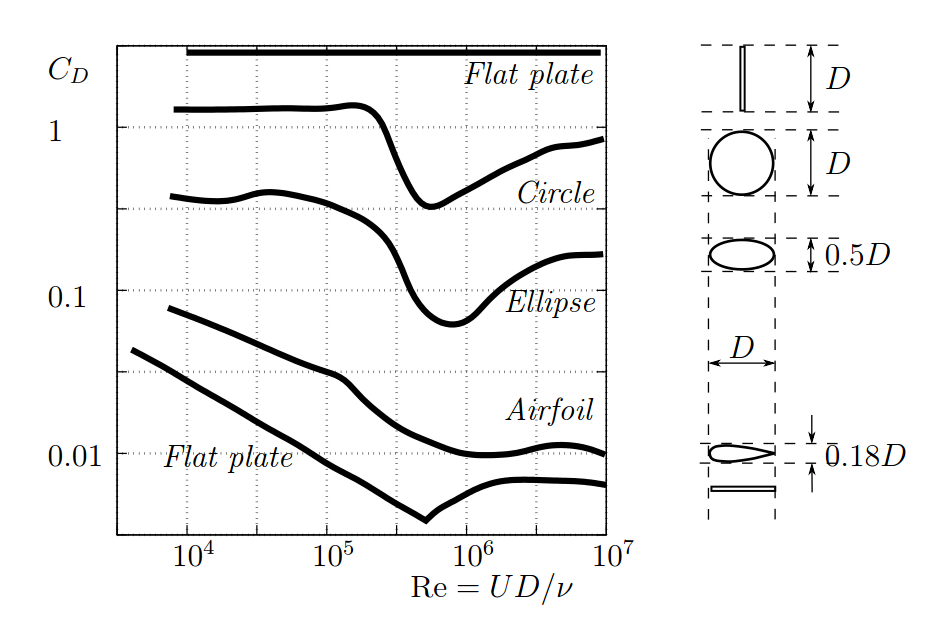
\includegraphics[width=.7\textwidth]{img/Cd_vs_Re.png}
    \caption{Drag coefficient $C_d$ as a function of the Reynolds number $Re$ for different shapes of the object.}
    \label{fig:velocity_inlet}
\end{figure}

From Figure \ref{fig:velocity_inlet} we can see that the drag coefficient $C_d$ changes significantly at low Reynolds numbers and has a drop across the transition from laminar to turbulent regime for non-slender bodies.

From a quick and approximated calculations we can clearly see that the rocket operate in the turbulence region for most of the flight duration, where the rate of change of the drag coefficient is less pronounced.
In particular, considering a set of velocities we can compute the Reynolds number $Re$ as:

\begin{equation}
    Re = \frac{\rho v L}{\mu} = \begin{cases}
        v = 110m/s \rightarrow Re = 4.9 \cdot 10^6 \\
        v = 50m/s \rightarrow Re = 2.2 \cdot 10^6  \\
        v = 10m/s \rightarrow Re = 4.5 \cdot 10^5  \\
    \end{cases}
\end{equation}

Where $\rho$ (density of the fluid) and $\mu$ (dynamic viscosity of the fluid) have been considered constant and equal to $1.225kg/m^3$ and $1.789 \cdot 10^{-5}kg/(m \cdot s)$ respectively.


\paragraph{Pressure outlet}

To set the pressure outlet inside the \texttt{Fluent} solver, we need to specify it as a gauge pressure.

For simplicity (and lack of experience with the software), we set the gauge pressure to $0Pa$.
This is equivalent to say that at the outlet boundary, the pressure is equal to the atmospheric pressure.

However, if we suppose that the atmospheric pressure considered by the software is the standard atmospheric pressure at sea level ($101325Pa$), this might result in a slight approximation of the simulation.

In fact, given that as stated in Table \ref{tab:conditions} the altitude of the starting point of the rocket is $1444m$ (meters above sea level), the atmospheric pressure is lower than the standard atmospheric pressure at sea level.
In particular, if we consider ideal gas law for the air flow, we can compute the atmospheric pressure at a given altitude as:

\begin{align}
    \frac{p}{\rho}                     & = \frac{RT}{M_{mol}}                                                   \\
    \frac{\nabla p}{p} = \nabla \ln(p) & = - \frac{g M_{mol}}{RT} \nabla \tilde{z}                              \\
    p                                  & = p_0 \exp\left(-\frac{g M_{mol} (\tilde{z} - \tilde{z_0})}{RT}\right)
    \label{eq:atmospheric_pressure}
\end{align}

Where $p$ is the pressure, $\rho$ is the density of the fluid, $R$ is the universal gas constant, $T$ is the temperature of the fluid, $M_{mol}$ is the molar mass of the fluid, $g$ is the acceleration due to gravity, $\tilde{z}$ is the altitude, $\tilde{z_0}$ is the altitude at the sea level and $p_0$ is the standard atmospheric pressure at sea level.

Given Equation \ref{eq:atmospheric_pressure}, we can compute the atmospheric pressure at the launch site, which is at an altitude of $1444m$, as:

\begin{equation}
    p_{launch} = 101325 \exp\left(-\frac{9.81 \cdot \frac{28.96}{1000} \cdot 1444}{8.31 \cdot (273.15 + 15)}\right) = 85378Pa
\end{equation}

We can see that at the launch site the atmospheric pressure is almost $16\%$ lower than the standard atmospheric pressure at sea level.

The difference is even more accentuated if we consider the altitude at the apogee of the rocket, which is around $1979m$.
In this case, the atmospheric pressure is:

\begin{equation}
    p_{apogee} = 101325 \exp\left(-\frac{9.81 \cdot \frac{28.96}{1000} \cdot 1979}{8.31 \cdot (273.15 + 15)}\right) = 80101Pa
\end{equation}

In this case, the atmospheric pressure is almost $21\%$ lower than the standard atmospheric pressure at sea level.

Given these considerations, we can imagine that the approximation of the atmospheric pressure at the outlet boundary of the domain might have a slight impact on the results of the simulations, forcing a small extra force from the bottom of the domain, resulting in a slight decrease of the velocity of the flow.
However, we believe that this approximation is not critical for the results of the simulations.


\subsection{Solver method}
\label{subsubsec:solver_method}

The last step in the setup of the \texttt{Fluent} solver is to set the solver method.

Thanks to knowledge acquired during the course, at this phase we were able to take informed decisions and we opted for the following settings:

\begin{table}[H]
    \centering
    \begin{tabular}{|c|c|}
        \hline
        \textbf{Parameter}       & \textbf{Value}      \\
        \hline
        Pressure-velocity scheme & Coupled             \\
        Momentum                 & Second Order Upwind \\
        \hline
    \end{tabular}
    \caption{Solver method settings used.}
    \label{tab:solver_method}
\end{table}

All the other parameters were left to the default settings, which for most of spatial discretization or interpolations schemes were set to \textit{Second Order Upwind}.

A complete list of the settings used for the simulations is reported in the \texttt{XML} file in the Appendix \ref{sec:appendix}.

\subsection{CFD results}
\label{subsec:cfd_results}

The simulation was run for $100$ iterations, which was enough to reach a good level of convergence considering the residuals and a converged value of the drag coefficient.

In particular, the final value of the drag coefficient was computed as $C_d = 0.86$.
This value is generally considered as almost out of the range of the drag coefficient for a rocket, which is usually between $0.7$ and $0.8$.
However, given the shape of the rocket and in particular the four fins that have a considerable impact on the drag coefficient, this value can be considered reasonable\footnote{We have runned multiple simulation varying of some perceptual point the velocity at the inlet, and we notice that the drag coefficient was extremely affected. We believe that this has something to do with an error in the simulation setup rather than a physical phenomenon.}.

\begin{figure}[H]
    \centering
    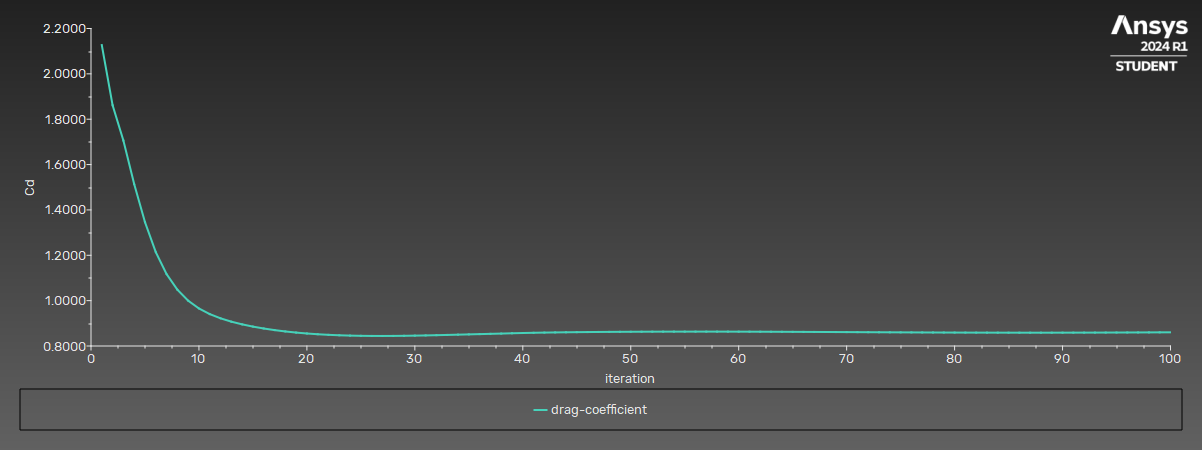
\includegraphics[width=.8\textwidth]{img/Results/Drag_coefficient_plot.png}
    \caption{Drag coefficient as function of the number of iterations.}
    \label{fig:drag_coefficient}
\end{figure}

\begin{figure}[H]
    \centering
    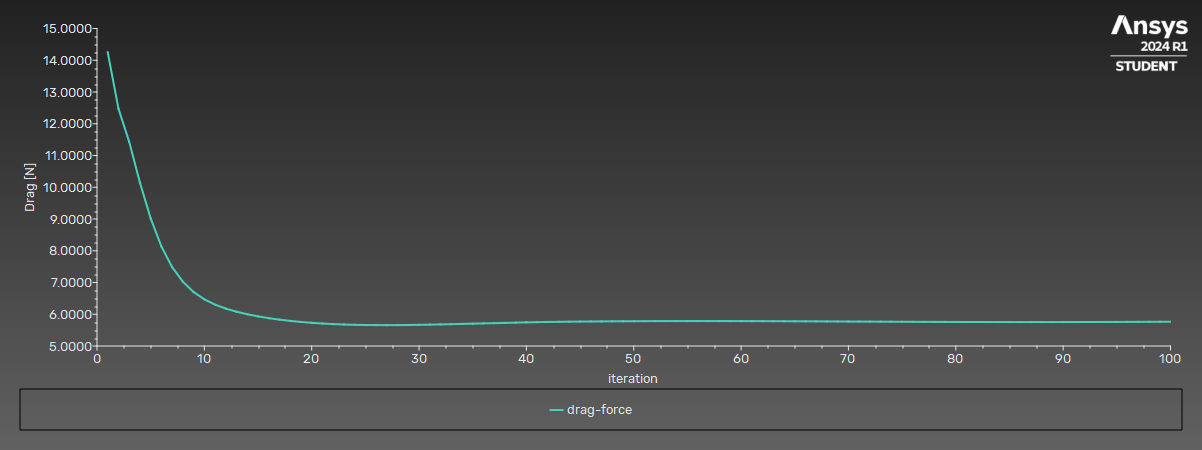
\includegraphics[width=.8\textwidth]{img/Results/Drag_force.png}
    \caption{Drag force as function of the number of iterations.}
    \label{fig:drag_force}
\end{figure}

\begin{figure}[H]
    \centering
    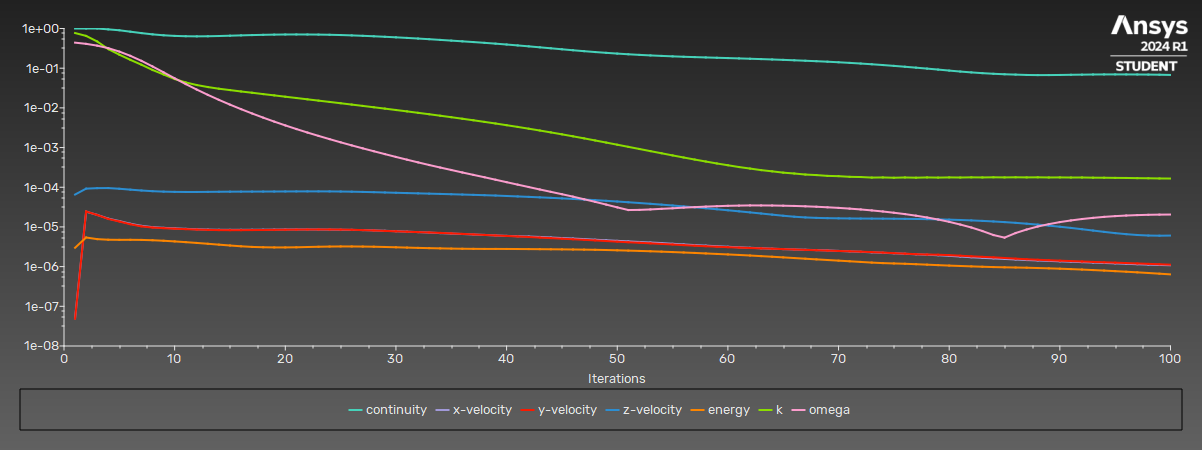
\includegraphics[width=.8\textwidth]{img/Results/Residuals_plot.png}
    \caption{Residuals as function of the number of iterations.}
    \label{fig:residuals}
\end{figure}


\subsubsection{Result visualization}
\label{subsubsec:result_visualization}

Although the main focus of the study was to compute the drag coefficient of the rocket, we can also proceed to analyze the pressure and velocity field around the rocket which can give us some insights on the flow field.

\paragraph{Pressure field}

Pressure contours around the rocket are shown in Figures \ref{fig:pressure_field} and \ref{fig:pressure_field_nose}.

\begin{figure}[H]
    \centering
    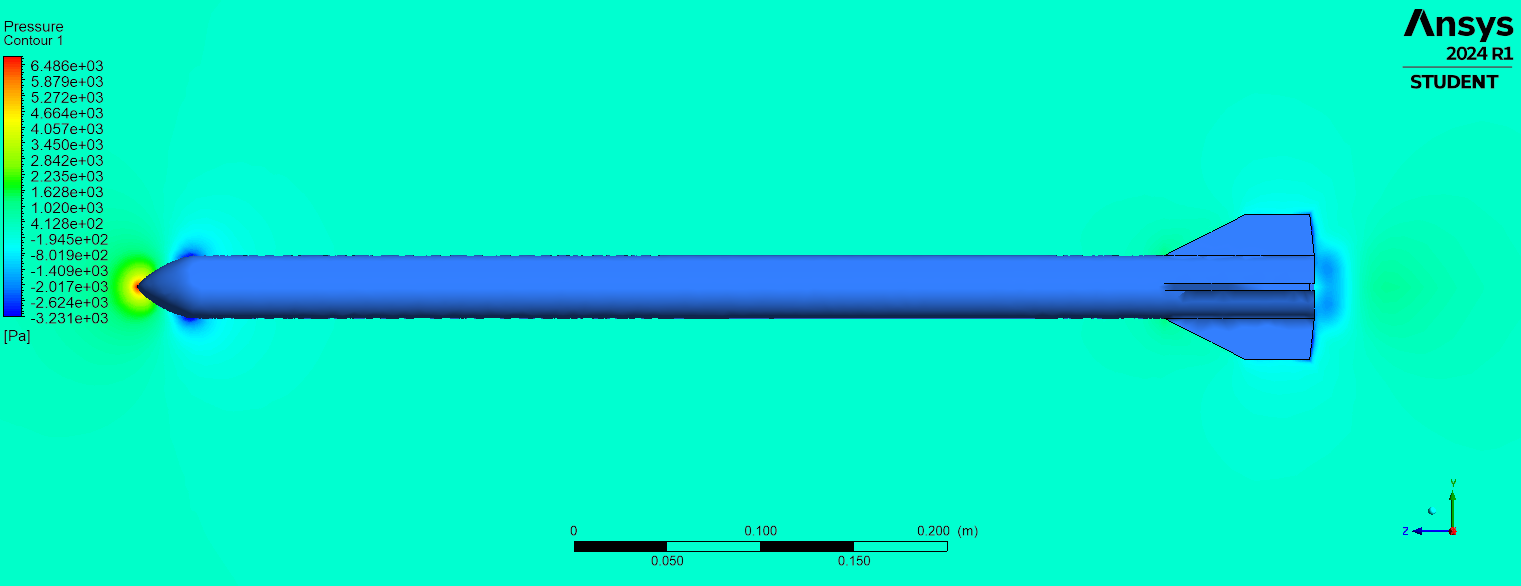
\includegraphics[width=.8\textwidth]{img/Results/Coutours_Pressure.png}
    \caption{Pressure contours around the rocket. Expected behavior is observed, with the pressure maximum at the bottom of the nose cone and the minimum at both the top of the nose cone. In the rear of the rocket, a low pressure area is formed even if not very pronounced.}
    \label{fig:pressure_field}
\end{figure}

\begin{figure}[H]
    \centering
    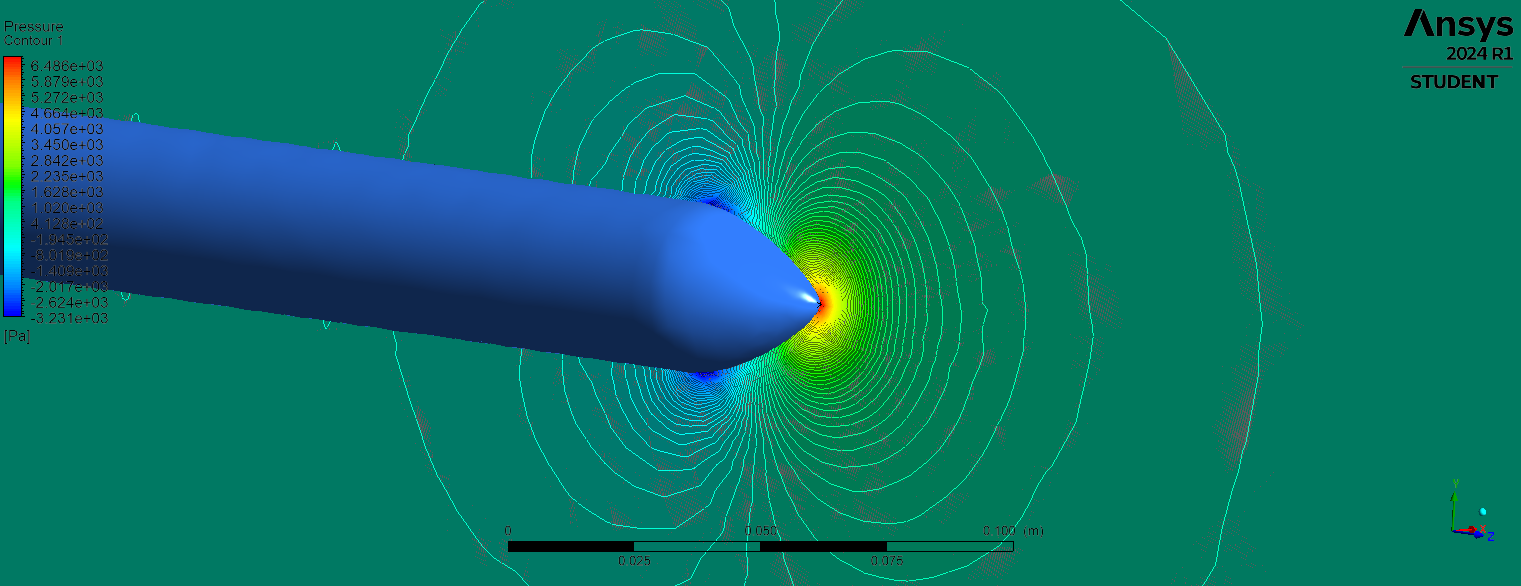
\includegraphics[width=.8\textwidth]{img/Results/Contours_Pressure_Nose.png}
    \caption{Detail of the pressure field around the nose cone.}
    \label{fig:pressure_field_nose}
\end{figure}


\paragraph{Velocity field}

Velocity contours and streamlines around the rocket are shown in Figures \ref{fig:velocity_field}, \ref{fig:velocity_field_nose} and \ref{fig:streamline_lateral}.

\begin{figure}[H]
    \centering
    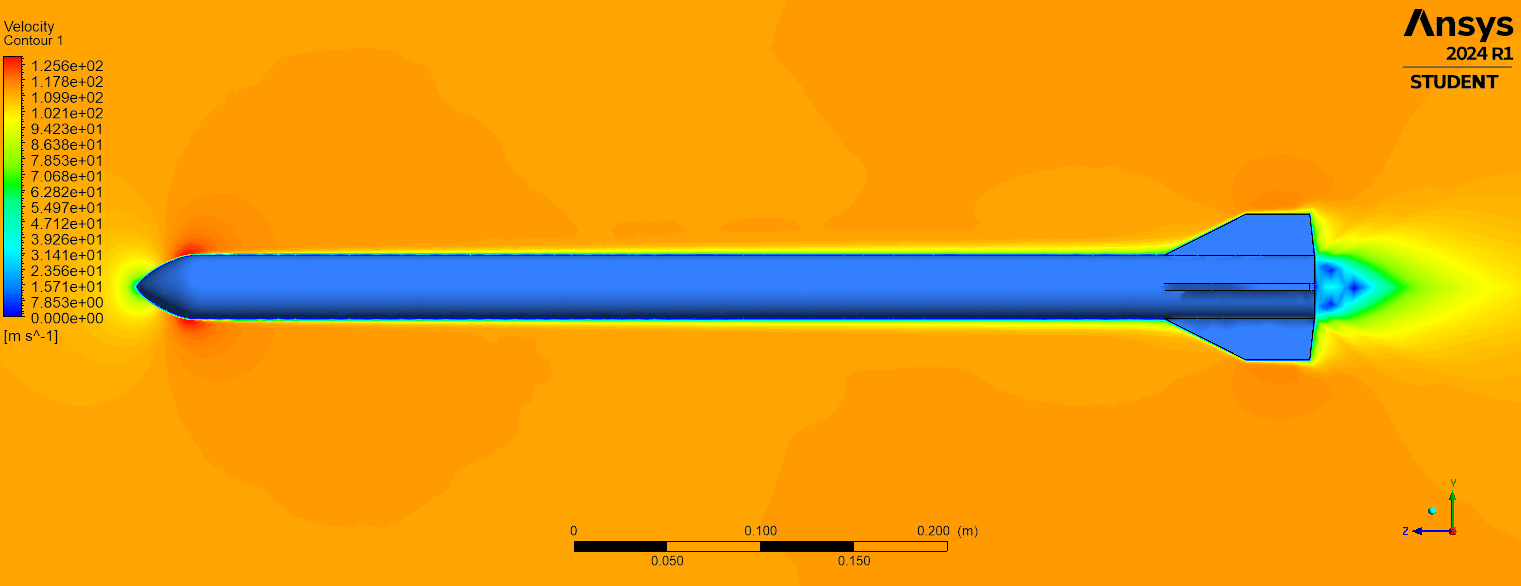
\includegraphics[width=.8\textwidth]{img/Results/Coutours_Velocity.png}
    \caption{Velocity contours around the rocket. Expected behavior is observed, with the velocity maximum at the bottom of the nose cone and the minimum at both the top of the nose cone and the rear of the rocket. No-slip condition are also respected.}
    \label{fig:velocity_field}
\end{figure}

\begin{figure}[H]
    \centering
    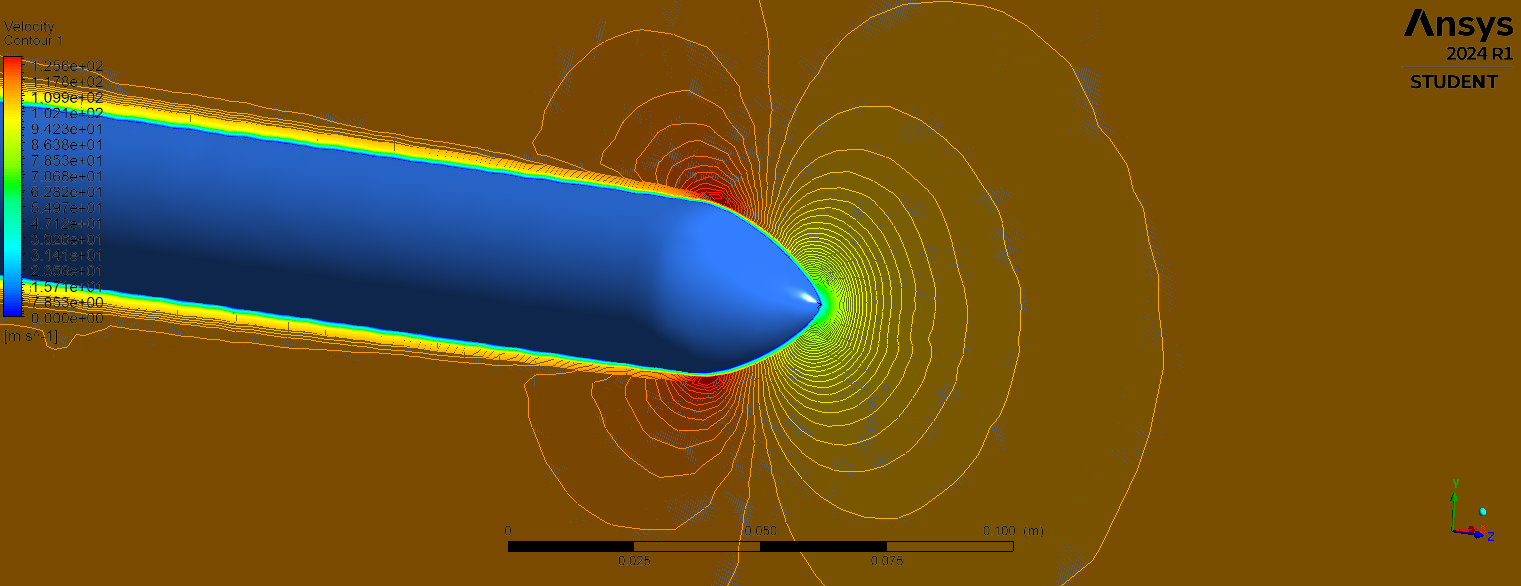
\includegraphics[width=.8\textwidth]{img/Results/Contours_Velocity_Nose.png}
    \caption{Detail of the velocity field around the nose cone.}
    \label{fig:velocity_field_nose}
\end{figure}

\begin{figure}[H]
    \centering
    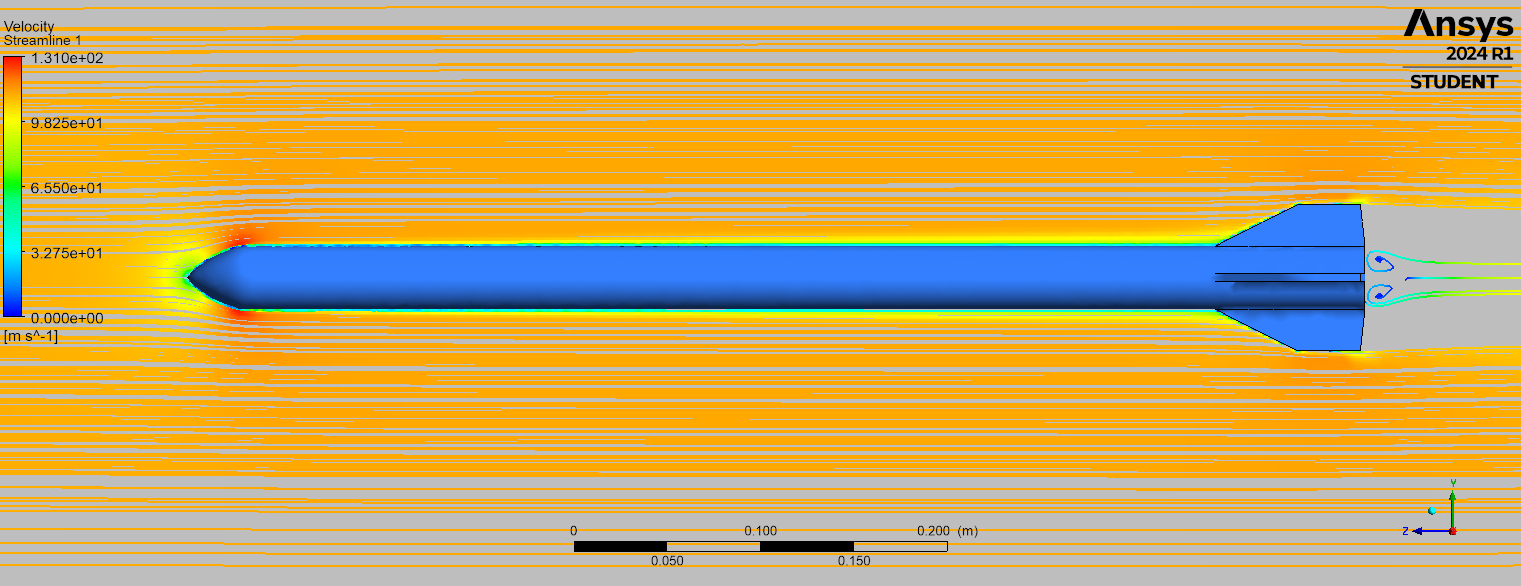
\includegraphics[width=.8\textwidth]{img/Results/Streamline_lateral.png}
    \caption{Streamlines around the rocket.}
    \label{fig:streamline_lateral}
\end{figure}


\paragraph{Vorticity field}

Vorticity streamlines are highlighted in Figure \ref{fig:vorticity_field}.

\begin{figure}[H]
    \centering
    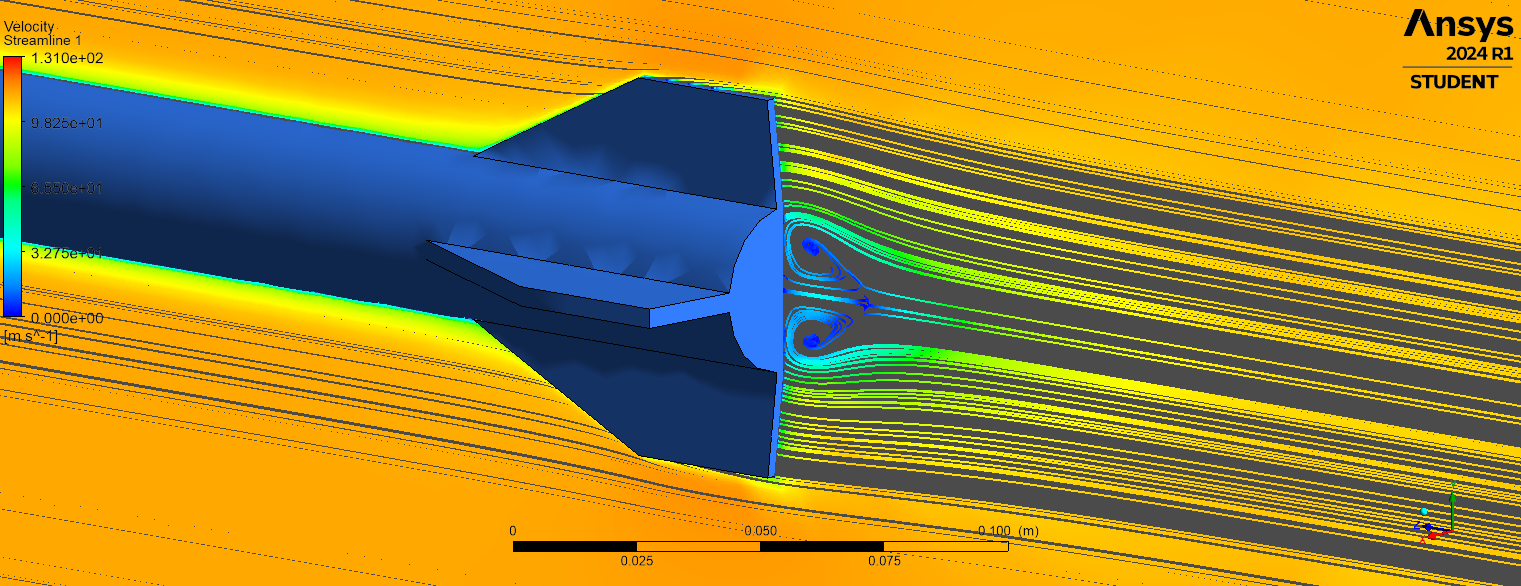
\includegraphics[width=.8\textwidth]{img/Results/Streamline_Fins.png}
    \caption{Vortex shedding behind the rocket are clearly visible.}
    \label{fig:vorticity_field}
\end{figure}


\paragraph{Temperature field}

Temperature contours around the rocket are shown in Figure \ref{fig:temperature_field}.

\begin{figure}[H]
    \centering
    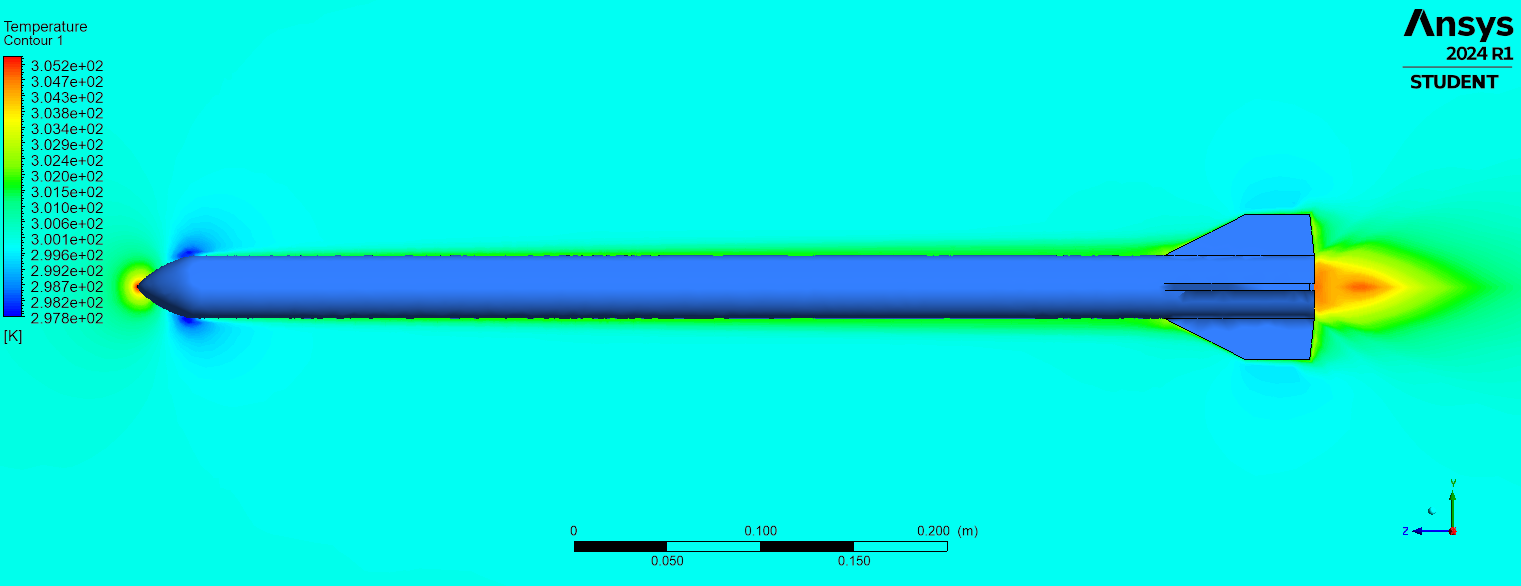
\includegraphics[width=.8\textwidth]{img/Results/Coutours_Temperature.png}
    \caption{Temperature field around the rocket. The variation is minimal ($+5 ^\circ C$ at the nose and $-2 ^\circ C$ at the first full cross-section of the body). It's interesting to see that the temperature rises also at the rear, where a vortex are formed.}
    \label{fig:temperature_field}
\end{figure}



\section{Analysis and validation of the results}
\label{sec:analysis_and_validation}

Finally, we can proceed with the validation of the results.

As previously mentioned in Section \ref{sec:methodology}, we are going to compare the results of the CFD simulations with both the flight data collected during the rocket launch and the results of the simulation run in \texttt{OpenRocket}.

To do so, we have coded in \texttt{MATLAB} a simple model that simulate the dynamics of the rocket flight, which takes into account drag force, gravity, thrust force and mass reduction due to the fuel consumption.

\subsection{Rocket flight physics model}
\label{subsec:rocket_flight_model}

To compute a simple flight dynamics model, it's necessary to observe the force acting on the rocket.
In Figure \ref{fig:forces_on_rocket}, the rocket is represented by a rectangle, and the forces acting on it are shown.

\begin{figure}[H]

    \centering
    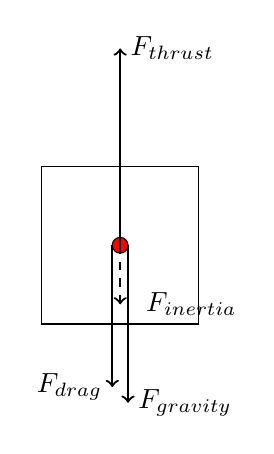
\begin{tikzpicture}

        \draw (0,0) rectangle (2, 2);

        \filldraw[fill=red, draw=black] (1, 1) circle (0.1);

        \draw[thick, ->] (1-0.1, 1) -- ++(0, -1.8) node[left] {$F_{\text{drag}}$};
        \draw[thick, ->] (1+0.1, 1) -- ++(0, -2) node[right] {$F_{\text{gravity}}$};
        \draw[thick, ->] (1, 1) -- ++(0, +2.5) node[right] {$F_{\text{thrust}}$};
        \draw[thick, ->, dashed] (1, 1) -- ++(0, -0.75) node[right=0.2cm] {$F_{\text{inertia}}$};

    \end{tikzpicture}
    \caption{Forces acting on the rocket during the flight.}
    \label{fig:forces_on_rocket}

\end{figure}

A simple balance of forces can be written as:

\begin{equation}
    F_{\text{thrust}} - F_{\text{drag}} - F_{\text{gravity}} = F_{\text{inertia}}
\end{equation}


\paragraph{Thrust force}

$F_{\text{thrust}}$ is the thrust force that the engine is supposed to deliver to the rocket during its flight.
In particular, knowing that the engine used for the rocket is a \texttt{TSP F35} engine, we can retrieve the thrust curve from the manufacturer's website obtaining the data shown in Figure \ref{fig:thrust_curve}.

\begin{figure}[H]
    \centering
    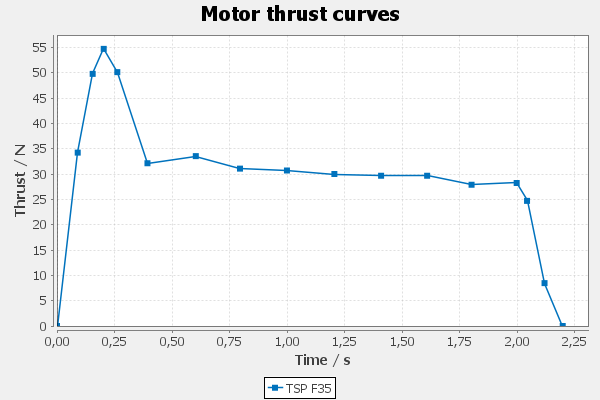
\includegraphics[width=.6\textwidth]{img/Thrust_curve.png}
    \caption{Thrust curve of the \texttt{TSP F35} engine.}
    \label{fig:thrust_curve}
\end{figure}

Equivalently, the thrust points are reported in Table \ref{tab:thrust_points}.

\begin{table}[H]
    \centering
    \begin{tabular}{|c|c|}
        \hline
        \textbf{Time [s]} & \textbf{Thrust [N]} \\
        \hline
        $0.000$           & $0.000$             \\
        $0.090$           & $34.235$            \\
        $0.155$           & $49.765$            \\
        $0.203$           & $54.706$            \\
        $0.262$           & $50.118$            \\
        $0.393$           & $32.118$            \\
        $0.603$           & $33.529$            \\
        $0.795$           & $31.059$            \\
        $0.999$           & $30.706$            \\
        $1.205$           & $30.000$            \\
        $1.408$           & $29.647$            \\
        $1.608$           & $29.647$            \\
        $1.801$           & $27.882$            \\
        $1.997$           & $28.235$            \\
        $2.042$           & $24.706$            \\
        $2.118$           & $8.471$             \\
        $2.197$           & $0.000$             \\
        \hline
    \end{tabular}
    \caption{Thrust points of the \texttt{TSP F35} engine.}
    \label{tab:thrust_points}
\end{table}

Given that we are going to solve the system at time step much more smaller than the time step of the thrust curve, we can interpolate the thrust curve to obtain the thrust force at each time step.

In the end, we can write:

\begin{equation}
    F_{\text{thrust}} = F_{\text{thrust}}(t_i) \approx F_{\text{thrust, interpolated}}(t)
\end{equation}


\paragraph{Drag force}

$F_{\text{drag}}$ is the drag force acting on the rocket during the flight.
This force can be computed as:

\begin{equation}
    F_{\text{drag}} = \frac{1}{2} \rho v^2 A C_d
\end{equation}

However, to more precise, we can also take into account some non-linearity of the equation such as the variation of the air density with respect to the altitude $\rho(\tilde{z})$ (see Equation \ref{eq:atmospheric_pressure}).
If this is the case, then the drag force can be computed as:

\begin{equation}
    F_{\text{drag}} = F_{\text{drag}}(\tilde{z}, v) = \frac{1}{2} \rho(\tilde{z}) v^2 A C_d
\end{equation}


\paragraph{Gravity force}

$F_{\text{gravity}}$ is the gravity force acting on the rocket during the flight.
This force can be computed as:

\begin{equation}
    F_{\text{gravity}} = m g
\end{equation}

However, it's important to notice that the mass of the rocket is not constant during the flight, but it's decreasing due to the fuel consumption.
In particular, knowing that the mass of the rocket at the beginning and at the end of the flight is $m_0 = 0.316kg$ and $m_f = 0.224kg$ respectively, we can compute the mass of the rocket function of time as:

\begin{equation}
    m(t) = \begin{cases}
        m_0 - \frac{m_0 - m_f}{t_f} t & \text{if } t \leq t_f \\
        m_f                           & \text{if } t > t_f
    \end{cases}
\end{equation}

Where $t_f$ is the time at which the engine stops working (see last row of Table \ref{tab:thrust_points}).

By doing so, the gravity force can be computed (neglecting any variation of the gravity with respect to the altitude) as:

\begin{equation}
    F_{\text{gravity}} = F_{\text{gravity}}(t) = m(t) g
\end{equation}


\paragraph{Inertia force}

$F_{\text{inertia}}$ is the inertia force acting on the rocket during the flight.
This force can be computed as:

\begin{equation}
    F_{\text{inertia}} = m(t) a(t)
\end{equation}

Where $a(t)$ is the acceleration of the rocket at time $t$.


\subsection{Equation of motion \& Code implementation}
\label{subsec:equation_of_motion}

By combining all the forces acting on the rocket, we can write the equation of motion as:

\begin{equation}
    m(t) \ddot{z} + \frac{1}{2} \rho(z) A C_d \dot{z}^2 + m(t) g = F_{\text{thrust}}(t)
    \label{eq:equation_of_motion}
\end{equation}

Where $z$ is the altitude of the rocket, $\dot{z}$ is the velocity of the rocket and $\ddot{z}$ is the acceleration of the rocket.

As often happen in mechanical problem, the equation of motion is a second-order differential equation.
To solve it, we can rewrite it as a system of first-order differential equations as:

\begin{equation}
    \begin{cases}
        \dot{z} = v \\
        \ddot{z} = \dot{v} = \frac{F_{\text{thrust}}(t) - \frac{1}{2} \rho(z) A C_d v^2 - m(t) g}{m(t)}
    \end{cases}
\end{equation}

The system of equations can be solved using a simple \texttt{MATLAB} script, which is reported in Listing \ref{lst:rocket_flight_model}.

\lstinputlisting[
    language=Matlab,
    caption={\texttt{MATLAB} script to compute the rocket flight model.},
    label={lst:rocket_flight_model},
]{files/rocket_flight_model.m}

The full version of the code can be found in the appendix (see Section \ref{sec:appendix}).
\subsection{CFD Simulation vs. Collected flight data \& \texttt{OpenRocket} simulation}
\label{subsec:cfd_vs_flight_data}

Finally, the results of the simulation are compared with the data collected during the rocket launch and the results of the simulation run in \texttt{OpenRocket}.

\subsubsection{Flight data}
\label{subsubsec:flight_data}

To collect data, we used a BMP280 barometer/thermometer sensor, which was placed inside the nose cone of the rocket and connected to an Arduino Nano board.
Because of poor quality SD writer module however, we weren't able to sampling at a high frequency and the number of collected data is limited (but still sufficient for our purpose).

In Table \ref{tab:flight_data} we report all the data collected during the rocket launch:

\begin{table}[H]
    \centering
    \begin{tabular}{|c|c|}
        \hline
        \textbf{Time [s]} & \textbf{Altitude [m]} \\
        \hline
        $494.130$         & $1443$                \\
        $495.233$         & $1443$                \\
        $496.334$         & $1444$                \\
        $497.437$         & $1554$                \\
        $498.540$         & $1678$                \\
        $500.745$         & $1809$                \\
        $501.848$         & $1847$                \\
        $502.953$         & $1903$                \\
        $504.055$         & $1931$                \\
        $505.161$         & $1958$                \\
        $506.263$         & $1973$                \\
        $507.364$         & $1979$                \\
        $508.468$         & $1976$                \\
        $509.570$         & $1965$                \\
        \hline
    \end{tabular}
    \caption{Data collected during the rocket launch.}
    \label{tab:flight_data}
\end{table}

In Figure \ref{fig:flight_data}, both the data of Table \ref{tab:flight_data} and their interpolation are shown.

\begin{figure}[H]
    \centering
    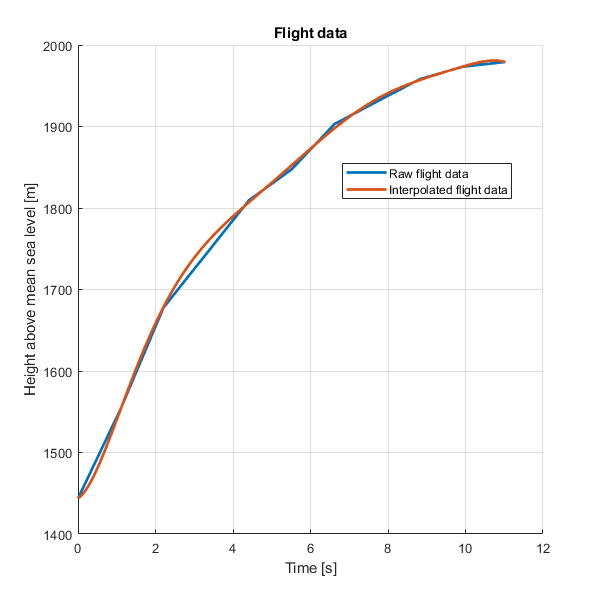
\includegraphics[width=.5\textwidth]{img/Validation/FlightData.png}
    \caption{Data collected during the rocket launch.}
    \label{fig:flight_data}
\end{figure}

For the interpolation, we used a Lagrange polynomial of degree $7$ (out of $10$ points) to obtain a smooth curve that can be used to compute also the vertical velocity of the rocket.


\subsubsection{\texttt{OpenRocket} simulation}
\label{subsubsec:openrocket_simulation}

As we have said, \texttt{OpenRocket} is a software that allows to both design and simulate the flight of a rocket.

By assigning shape, dimensions, mass, and an hypothetical $C_d$ to each component of the rocket, the software is able to give a raw estimation of the dynamics during the flight.
In Figure \ref{fig:openrocket_simulation}, the results of the simulation run in \texttt{OpenRocket} are shown.

\begin{figure}[H]
    \centering
    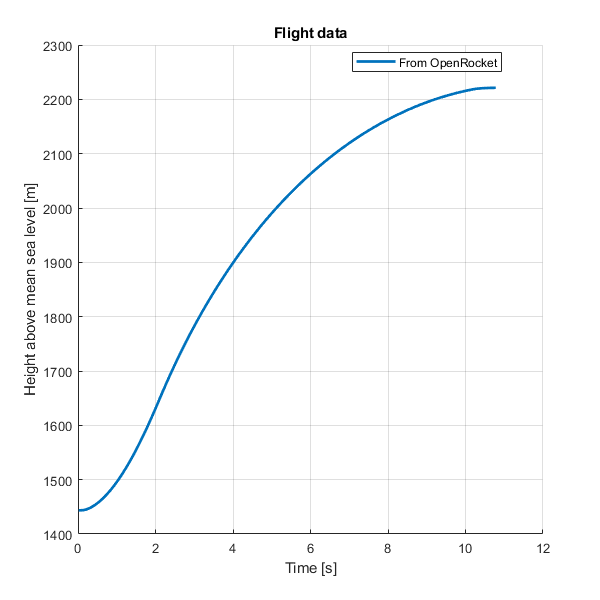
\includegraphics[width=.5\textwidth]{img/Validation/OpenRocket.png}
    \caption{Simulation run in \texttt{OpenRocket}.}
    \label{fig:openrocket_simulation}
\end{figure}


\subsubsection{Final comparison}
\label{subsubsec:final_comparison}

From Figure \ref{fig:flight_data} and Figure \ref{fig:openrocket_simulation}, we can see that the two curves (at the least in the apogee altitude) are not in agreement.

This is a common situation, as the simulation in \texttt{OpenRocket} are performed considering almost ideal condition and neglecting any possible aerodynamic imperfection of the rocket (which of course are present in the real world).

To overcome this discrepancy between the simulation and the real world, we will decrease the thrust curvature by a given factor until the peak velocity between the two curves are the same.
This might be a very strong assumption, but in reality in the world of model rocket is quite common as the effective thrust of the engine is almost always lower than the nominal thrust declared by the manufacturer.

Having said this, we can proceed with the comparison of the results of the CFD simulation with the collected flight data.

\paragraph{CFD simulation vs. \texttt{OpenRocket} simulation}

In Figure \ref{fig:comparison_flight_data}, the altitude and the vertical velocity of the rocket are shown.

\begin{figure}[H]
    \centering
    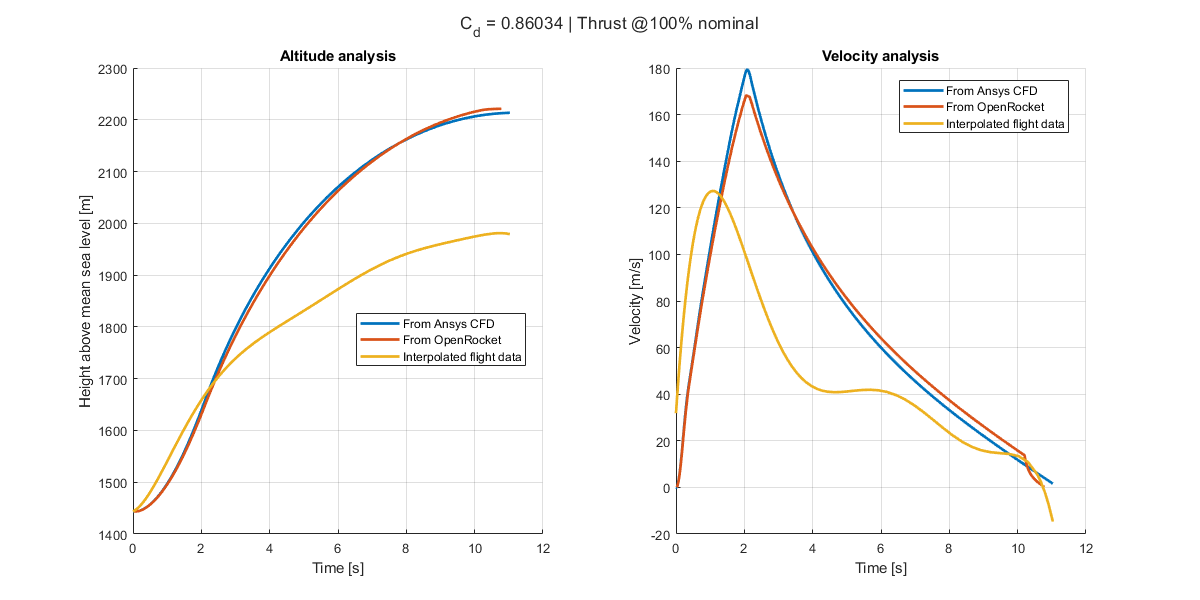
\includegraphics[width=\textwidth]{img/Validation/All_100.png}
    \caption{
        Comparison of the altitude and the vertical velocity of the rocket, considering a full thrust curve and $C_d = 0.86$ (from the CFD simulation).
        As the legend reports, the blue line represents the prediction based on the $C_d$ computed in the CFD simulation, the orange line represents the simulation run in \texttt{OpenRocket}, while the yellow line represents the collected flight data.
    }
    \label{fig:comparison_flight_data}
\end{figure}

As we can see, the curves generated with the CFD simulation and the one from \texttt{OpenRocket} are almost identical, while the collected flight data are way off.

\paragraph{CFD simulation vs. collected flight data}

However, as we have mentioned at the beginning of this section, the thrust curve of the engine are usually not accurate and often turns out to be much less than the nominal thrust declared by the manufacturer.
To overcome this discrepancy, we can decrease the thrust curve by a factor of $0.7$ until the peak velocity between the flight data and the CFD simulation are the same.
In this case, the results are shown in Figure \ref{fig:comparison_flight_data_70}.

\begin{figure}[H]
    \centering
    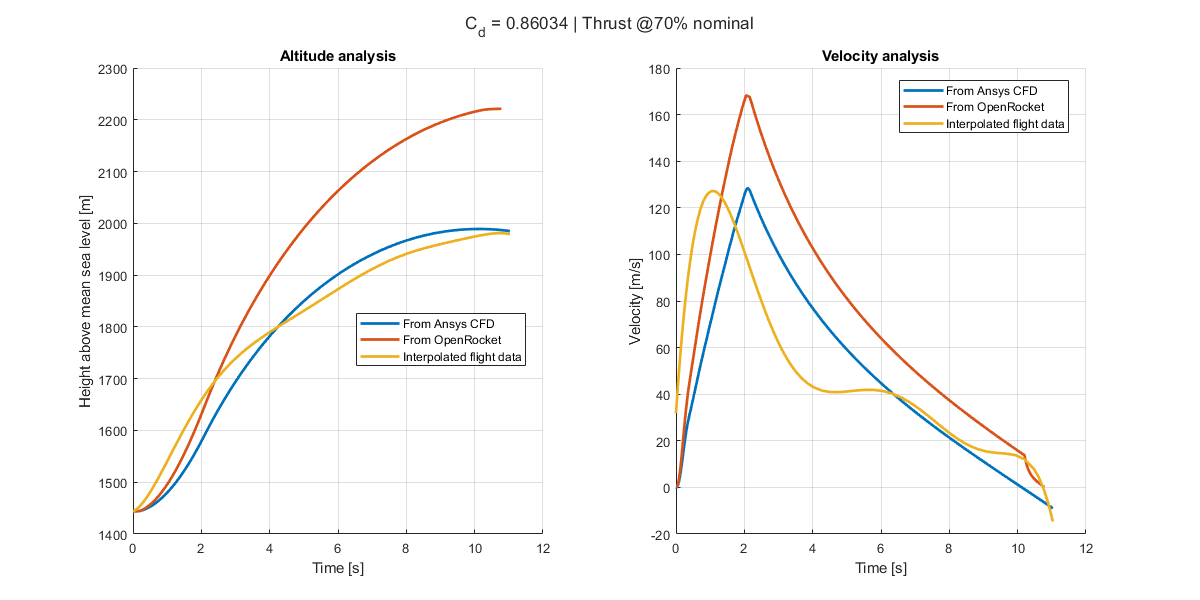
\includegraphics[width=\textwidth]{img/Validation/All_70.png}
    \caption{Comparison of the altitude and the vertical velocity of the rocket, considering a thrust curve decreased by a factor of $0.7$ and $C_d = 0.86$ (from the CFD simulation).}
    \label{fig:comparison_flight_data_70}
\end{figure}

By decreasing the thrust curve by a factor of $0.7$, the peak velocity of the flight data and the CFD simulation are almost the same.
Even if collected data are few and of poor quality (see the strong non-physical oscillation in the velocity curve), we can still try to relate the two curves.
By doing so, we can see that the CFD simulation is in good agreement with the collected data, while the simulation run in \texttt{OpenRocket} of course is not.

\paragraph{\texttt{OpenRocket} coefficient of drag estimation}

One may also ask what's the coefficient of drag used in the \texttt{OpenRocket} simulation.
Unfortunately, the software doesn't provide this information, but we can try to estimate it by comparing the altitude estimation for different values of $C_d$ around the value computed in the CFD simulation.
In Table \ref{tab:openrocket_cd}, we report three different values of $C_d$ and the corresponding peak altitude and velocity computed using our simple model and the comparison with the simulation from \texttt{OpenRocket}.

\begin{table}[H]
    \centering
    \begin{tabular}{|c|c|c|}
        \hline
        $C_d$               & \textbf{Altitude @ $t=10s$ [m]} & \textbf{Peak velocity [m/s]} \\
        \texttt{OpenRocket} & $2.2166e+03$                    & $168.2810$                   \\
        $0.903$             & $2.1900e+03$                    & $177.6557$                   \\
        $0.860$             & $2.2068e+03$                    & $179.3001$                   \\
        $0.817$             & $2.2271e+03$                    & $180.9773$                   \\
        \hline
    \end{tabular}
    \caption{Comparison of the peak altitude and velocity for different values of $C_d$.}
    \label{tab:openrocket_cd}
\end{table}

In Table \ref{tab:openrocket_cd}, we presented the results for $C_d = 0.903$, $C_d = 0.860$ and $C_d = 0.817$ (that are respectively $5\%$ and $5\%$ lower and higher than the value computed in the CFD simulation).
As we can observe, the peak velocity is almost the same for the three values of $C_d$, while the peak altitude is slightly different.
In particular, the best correspondence with the \texttt{OpenRocket} simulation is obtained for $C_d = 0.860$.
Also, from a shape point of view, the curve obtained with $C_d = 0.860$ is the one that best fits the \texttt{OpenRocket} simulation.


\section{Conclusions}
\label{sec:conclusions}

The present work aimed at investigating the drag coefficient of a model rocket using computational fluid dynamics.

The rocket was at first modeled in an external CAD software and then imported into Ansys Fluent for the CFD simulation.
The simulation was carried out using the $k-\omega$ SST turbulence model and in a steady-state regime and the drag coefficient ($C_d$) was calculated at $85\%$ of the speed maximum speed reached by the rocket during the real world flight.

The results obtained from the CFD simulation were compared to the flight data and the simulation from \texttt{OpenRocket}, showing a good agreement with both of them after some adjustments to the thrust curve.

Moreover, the drag coefficient was found to be $C_d = 0.86$, which is in line with the expected values for a model rocket.
This value is also in line with the one obtained from the flight data and the one from \texttt{OpenRocket}.

The present work showed that CFD simulations can be a powerful tool to investigate the aerodynamic behavior of model rockets and that the results obtained can be potentially used to optimize the design iterating backward and forward between the CAD model and the CFD simulation.


\clearpage
\bibliographystyle{plain}
\bibliography{references}


\clearpage
\appendix
\label{sec:appendix}

\section{\texttt{Ansys Fluent} settings for the CFD simulation}
\lstinputlisting[
	style=XML,
	language=XML,
	caption=Settings applied to the CFD simulation in \texttt{Ansys Fluent}.,
]{files/report.xml}

\section{\texttt{MATLAB} code used for the validation phase}
\lstinputlisting[
	language=Matlab,
	caption=\texttt{MATLAB} code used for validating the CFD simulation result against flight data and simulation from \texttt{OpenRocket}.,
]{files/Main.m}


\end{document}
